\part{Pruebas del software}

\section{Introducción}

Una de las características típicas de los ciclos de vida en el desarrollo de software es la realización de controles periódicos, con el objetivo de evaluar la calidad de los productos generados, y poder \textbf{detectar así fallos en ellos cuanto antes}. Aún así, todo sistema/aplicación debe ser \textbf{probado}, independientemente de estas revisiones, mediante su \textbf{ejecución controlada antes de ser entregado al cliente}; estas se denominan habitualmente como \uline{pruebas}.\\

Las pruebas permiten verificar y validar el software; cabe recordar el significado de estos dos términos:

\begin{itemize}
    \item \textbf{Verificación} (pruebas de \uline{caja blanca}): Proceso de evaluación de un sistema o de uno de sus componentes para determinar si los productos de la fase sobre el que se realiza satisfacen las condiciones impuestas al principio de esta fase. Dicho de otro modo, se puede decir que se pregunta \uline{si se está construyendo correctamente el producto}.
    
    \item \textbf{Validación} (pruebas de \uline{caja negra}): Proceso de evaluación del sistema o de uno de sus compoentes para determinar, bien sea durante o al final del desarrollo, si satisface los requisitos especificados. Dicho de otro modo, se puede decir que se pregunta \uline{si se está construyendo el producto correcto}.
\end{itemize}

Como se puede ver, el contar con la posibilidad de enfocar las pruebas hacia cualquiera de estos dos puntos de vista permite enfrentar cualquier fase del ciclo de vida a:

\begin{itemize}
    \item La metodología de la propia fase: Verificación.
    \item Los requisitos: Validación.
\end{itemize}

\section{Definiciones}

El \textit{IEEE} propone, entre otras, las siguientes definiciones en relación a las pruebas.

\paragraph{Pruebas} Actividad en la que un sistema o uno de sus componentes se ejecuta en circunstancias previamente especificadas, y cuyos resultados son observados, registrados y evaluados comprobando algún aspecto determinado de antemano. \textit{Proceso de ejecutar un programa con el fin de encontrar errores.}\\

Una prueba consta de uno o más casos de prueba.

\paragraph{Caso de prueba} Conjunto de entradas, condiciones de ejecución y resultados esperados desarrollados para un objetivo particular. \textit{Por ejemplo: ejercitar un camino concreto de un programa, o verificar el cumplimiento de un determinado requisito.}\\

Por extensión, un caso de prueba válido debe comprobar que se deja hacer lo que se debería, y que no se permite hacer lo que no. Además, un buen caso de prueba es aquel que tiene una \uline{alta probabilidad de detectar un error}.\\

\textbf{Nota:} \textit{Por ejemplo, una prueba del módulo de menús de un software para comedores constaría de varios casos de prueba; estos podrían ser que un jefe de una cafetería pueda \{insertar, borrar, modoficar\} un menú.}

\paragraph{Defecto} Incorrección en el software que \textbf{genera un fallo}. \textit{Por ejemplo: un proceso, una definición de datos o un paso de procesamiento incorrectos en un programa.}

\paragraph{Fallo} Incapacidad de un sistema o de alguno de sus componentes para realizar las funciones requeridas dentro de los requisitos de rendimiento especificados. \textit{Es el hecho de que el software no pueda funcionar.}

\textbf{Nota:} \textit{Un fallo causado por un defecto es culpa de los desarrolladores, mientras que un fallo sin defecto es culpa del entorno, al poder presentar características como ser altamente cambiante. Por este motivo, es importante concretar un entorno para las pruebas, así como replicar las condiciones en las que el software será explotado.}

\paragraph{Error} Presenta varias acepciones:
\begin{itemize}
    \item Diferencia entre un valor calculado, observado o medido y el valor verdadero, especificado o teóricamente correcto.
    \item Resultado incorrecto.
    \item Defecto en el software.
    \item Acción humana que conduce a un resultado incorrecto.
\end{itemize}

\begin{figure}[H]
    \centering
    \includegraphics[width=0.8\linewidth]{Resources/cuernos}
    \caption{Recuerda: error, defecto y fallo no son lo mismo. Al final, se provocan efectos negativos.}
    \label{fig:cuernos}
\end{figure}


\section{Filosofía de las pruebas del software}

Las características especiales del software, como que carezca de leyes que rijan su comportamiento, o presentar una gran complejidad habitualmente, hacen aún más difícil la tarea de probarlo, de modo que la \textbf{prueba exhaustiva del software es impracticable}: \textbf{no} se pueden probar todas las posibilidades incluso en programas pequeños y sencillos. Además, esta situación se ve empeorada por la presencia de preujicios y por la habitual falta de tiempo en el desarollo del proyecto. Por ello, es interesante estudiar cuál es la mejor actitud a seguir en esta actividad; en general, será interesante \uline{sistematizar todo lo posible} de las pruebas, para ahorrar en tiempo y recursos.\\

Es necesario, en primer lugar, un fuerte cambio de mentalidad, dejando atrás la visión constructiva del desarrollo del software, para dar paso a la \uline{visión destructiva} de intentar tirar abajo lo construido. Al final el objetivo de las pruebas, desde el punto de vista del proyecto, es la detección de defectos en el software, por lo que \textbf{el descubrir un defecto debe considerarse como el éxito de una prueba}.\\

En segundo lugar, también es necesario tener presente que todo el mundo comete errores, por lo que no hay que sentirse culpable por haber encontrado una metedura de pata; desde luego, es mejor que el desarrollador se encuentre con un fallo, en lugar de que tenga que ser reportado por el cliente. Es más, los defectos no son siempre el resultado de la negligencia, sino que influyen múltiples factores en su aparición, como la mala comunicación entre los miembros del equipo, que da lugar a malentendidos.\\

Además del objetivo mencionado anteriormente, también cabe destacar que el objetivo de las pruebas, pero ahora desde el punto de vista de ser un proceso, es el \textbf{diseñar técnicas que permitan un desarollo sistemático de pruebas} para garantizar ese primer objetivo; es en esta visión en la que se centrará el documento.\\

Finalmente, la realización de pruebas en el software también cuenta con determinadas ventajas secundiarias:

\begin{itemize}
    \item \textbf{Demuestran hasta qué punto se verifican los requisitos:} No siempre va a ser posible satisfacer todos; por ejemplo, es posible que queden en ``segundo plano'' los requisitos estimulantes (quedarían bien), o incluso podrían verse afectados requisitos más relevantes por limitaciones de tiempo y de recursos, agravados aún más en el caso de que se produzcan cambios en los requisitos durante el desarrollo del proyecto.
    \item \textbf{Se generan datos de prueba que informan sobre la fiabilidad del software.}
\end{itemize}

\textbf{Nota:} \textit{La realización de pruebas no asegura la ausencia de fallos; pero, el descubrimiento de un defecto, significa un éxito para la mejora de la calidad.}\\

\textbf{Nota:} \textit{A veces, no será posible subsanar todos los errores encontrados por limitaciones de tiempo y de recursos. En estos casos, es necesario discernir entre qué errores se corregirán y cuáles no; por ejemplo, no se conrregirán aquellos que fallen en menos del 10\% de los tests.}

\subsection{Principios}

Los seis primeros fueron enunciados por \textit{Davis}, y los restantes por \textit{Myers}; a estos últimos, es además necesario incluir de nuevo el principio de Pareto, y que el grupo de pruebas deba ser independiente del de programación.

\begin{enumerate}
    \item \textbf{A todas las pruebas se les debería poder hacer un seguimiento hasta los requisitos del cliente}. Se logra mediante la \uline{trazabilidad}:
    \begin{itemize}
        \item Trazabilidad hacia arriba: Si se detecta un fallo, es posible identificar a qué requisitos afecta para evaluar si compensa o no solventarlo.
        \item Trazabilidad hacia abajo: Si se produce un cambio en un requisito, qué pruebas es necesario cambiar para poder validar este nuevo requisito.
    \end{itemize}
    \item \textbf{Las pruebas deberían planificarse mucho antes de que empiecen, y ser repetibles} (probar $\rightarrow$ corregir, probar $\rightarrow$ corregir\ldots): La planificación de pruebas puede comenzar tan pronto como esté completo el modelo de requisitos. La definición detallada de los casos de prueba puede empezar tan pronto como el modelo de diseño se haya consolidado. Como se puede ver, es posible planificar y diseñar algunas pruebas incluso antes de generar ningún código.
    \item \textbf{El 80\% de los errores surgen al hacer el seguimiento del 20\% de los módulos del Software (\textit{Principio de Pareto})}: Conviene aislar los módulos sospechosos.
    \item \textbf{Las pruebas tendrían que hacerse de lo pequeño hacia lo grande}: En caso contrario, será difícil concretar el origen de los problemas.
    \item \textbf{No son posibles pruebas exhaustivas, ni probar todo al mismo tiempo}. Sin embargo, es posible cubrir adecuadamente la lógica del programa y asegurarse de que se han aplicado todas las condiciones en el diseño a nivel de componente.
    \item \textbf{Las pruebas deberían ser realizadas por un equipo independiente del de desarrollo}: El haber sido el responsable de la construcción del software probablemente lleve a realizar pruebas menos rigurosas, así como es habitual que condiciones que se olvidaron al crear el programa vuelvan a ser obviadas al escribir casos de prueba (por ejemplo, que se reciba un fichero vacío).
    \item \textbf{Cada caso de prueba debe definir el resultado de salida esperado} y compararlo con el realmente obtenido.
    \item \textbf{Se debe inspeccionar a conciencia el resultado de cada prueba}, para así poder descubrir posibles síntomas de defectos.
    \item \textbf{Al generar casos de prueba se deben incluir tanto datos de entrada válidos y esperados, como no válidos e inesperados.}
    \item \textbf{Las pruebas deben centrarse en probar si el software}:
          \begin{itemize}
              \item \textbf{No hace lo que debe hacer}.
              \item \textbf{Hace lo que no debe hacer}.
          \end{itemize}
    \item \textbf{Se deben evitar los casos desechables}; es decir, los no documentados o diseñados sin cuidado: Como suele ser necesario probar una y otra vez el software, el no documentar o no guardar los casos significa repetir constantemente el diseño de casos de prueba. \textit{Por ejemplo, se incluirían aquí las pruebas tecleadas sobre la marcha.}
    \item \textbf{No deben hacerse casos de prueba suponiendo que no hay defectos en los programas}: Dicho de otro modo, no deben dedicarse pocos recursos a las pruebas.
    \item \textbf{Las pruebas son una tarea tanto o más creativa que el desarrollo de software}: Dado que no existen técnicas rutinarias para concebirlas.
\end{enumerate}

Una vez visto todo esto, se puede concluir que la filosofía más adecuada consiste en planificar y diseñar las pruebas de forma sistemática para poder detectar el máximo número y variedad de defectos con el mínimo consumo de tiempo y esfuerzo. Es también necesario recordar que un buen caso de prueba es aquel que tiene una gran probabilidad de encontrar un defecto no descubierto aún, y que el éxito de una prueba consiste en detectar un defecto no encontrado antes.


\section{El proceso de prueba}

En la siguiente figura, se puede ver una representación del proceso completo relacionado con las pruebas basada, en parte en el estándar, y en parte en \textit{Pressman}. En este documento, no se hará más énfasis en él.

\begin{figure}[H]
    \centering
    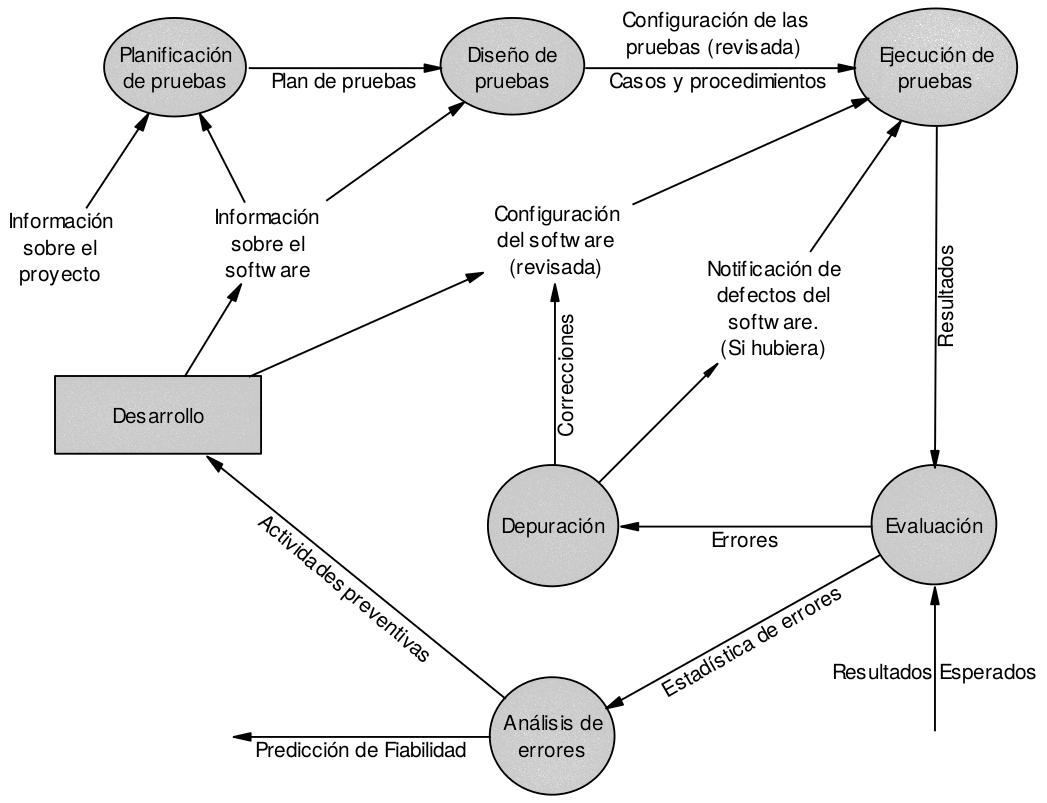
\includegraphics[width=0.8\linewidth]{Resources/Tema6/ProcesoPruebas_IEEE_Pressman.png}
    \caption{Proceso relacionado con las pruebas según el estándar y según \textit{Pressman}. Las flechas entrantes en cada actividad representan información de entrada requerida para su realización.}
\end{figure}


\section{Técnicas de diseño de casos de prueba}

Como se comentó anteriormente, el diseño de casos de prueba está totalmente condicionado por la imposobilidad de probar exhaustivamente el software. Por ello, las técnicas de diseño de casos de prueba tienen como objetivo \textbf{conseguir una confianza aceptable en la que se detectarán los efectos existentes}, al no ser obtenible la seguridad total, \textbf{sin consumir una cantidad excesiva de recursos}. Alcanzar un equilibrio entre dicha confianza y el uso de recursos no es sencillo cuanto menos.\\

La idea fundamental para el diseño de casos de prueba es \textbf{elegir algunas de ellas que, por sus características, se consideren representativas del resto}; de este modo, se asume que, si no se detectan defectos en el software al ejecutar dichos casos, se puede contar con un cierto nivel de confianza en que el programa no tiene defectos. Es necesario recurrir a ciertos criterios de elección para construir los mejores casos de prueba posibles, como preguntase cómo puede fallar el software, escoger casos no redundantes, que no sean ni demasiado sencillos ni demasiado complejos\ldots\\

Existen dos enfoques principales:

\begin{enumerate}
    \item \textbf{Estructural o de caja blanca} (verificación): Consiste en centrarse en la estructura interna (implementación) del programa, realizando pruebas que aseguren que todos los módulos o componentes internos funcionan bien y encajan correctamente. \textit{La prueba exhaustiva consistiría en probar todos los posibles caminos de ejecución.}
    \item \textbf{Funcional o de caja negra} (validación): Consiste en estudiar la especificación de las funciones (interfaz), dejando de importar cómo está implementada la aplicación. De esta especificación, se derivan los casos, probándose que cada función es completamente operativa puesto que se conoce qué es lo que debe realizar. \textit{La prueba exhaustiva consistiría en probar todas las posibles entradas y salidas del programa.}
\end{enumerate}

Cabe destacar que estos enfoques no son excluyentes, sino que \textbf{son complementarios}. Por ejemplo, podrían diseñarse inicialmente los casos de prueba de caja negra y, a la hora de diseñar los de caja blanca, cabría la posibilidad de que algunos casos de estos últimos ya estuviesen cubiertos; al final, es necesario que se recorran determinados caminos en la ejecución de las pruebas de caja negra.


\section{Pruebas estructurales (de caja blanca)}

Es interesante realizar pruebas de caja blanca porque:

\begin{itemize}
    \item Los errores tipográficos son aleatorios, por lo que pueden aparecer en cualquier parte del programa, se ejecute regularmente o no.
    \item Se suele creen que un determinado flujo es poco probable cuando, de hecho, puede ejecutarse regularmente.
    \item En relación al anterior punto, en general, la probabilidad e importancia de un trozo de código suelen ser calculadas de forma muy subjetiva. \textit{Por ejemplo, si el programador sabe que un camino probablemente se ejecute poco, es probable que le preste menos atención que a otros, incrementándose por lo tanto la probabilidad de que se encuentren errores en él.}
\end{itemize}

El diseño de casos de prueba tiene que basarse en la \textbf{elección de caminos importantes que ofrezcan una seguridad aceptable de descubrir un defecto}, y para ello se utilizan los criterios de cobertura lógica. No requieren el uso de representaciones gráficas, pero se suelen utilizar grafos de flujo (estrechamente relacionados con los diagramas de flujo de control), con el objetivo de \uline{convertir el código en un grafo y facilitar así la visualización de sus posibles caminos}.

\begin{figure}[H]
    \centering
    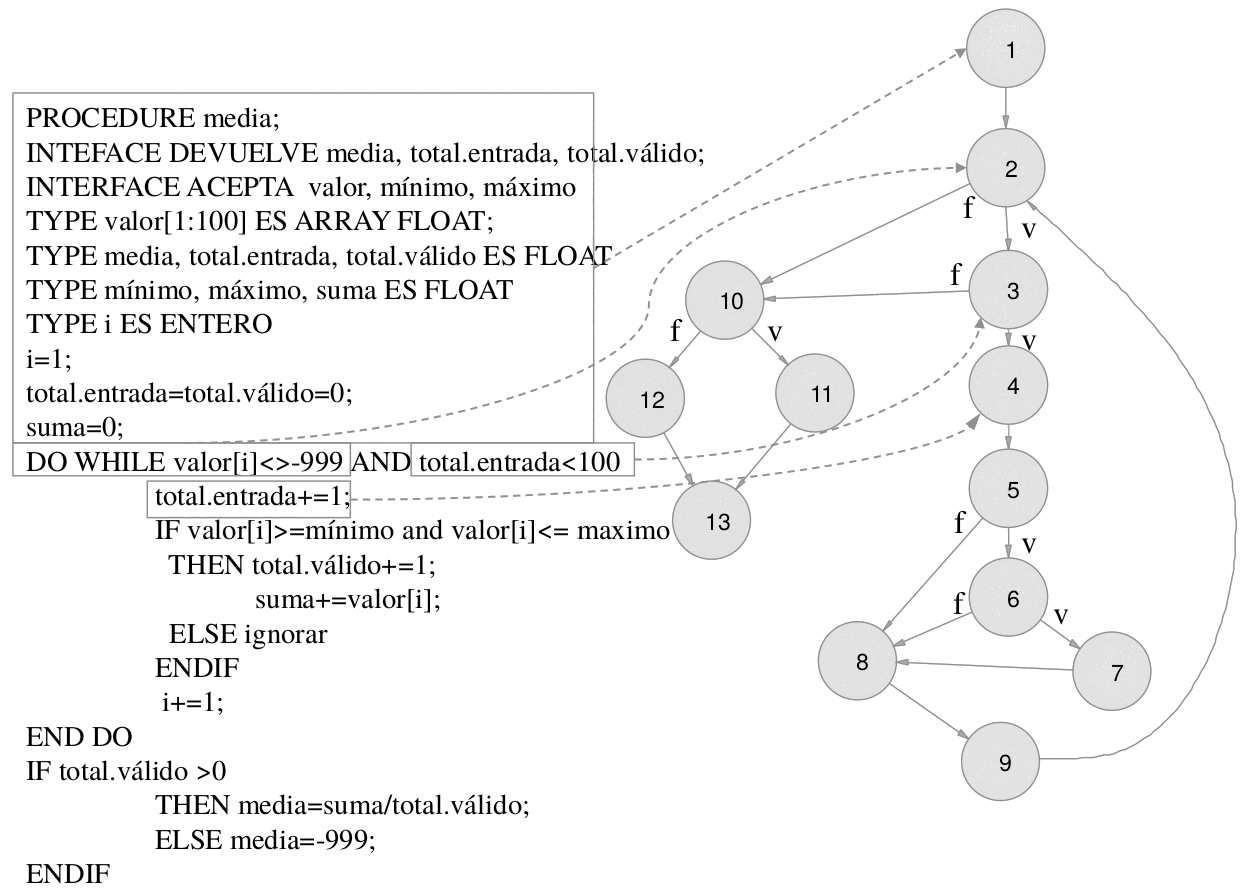
\includegraphics[width=0.8\linewidth]{Resources/Tema6/Ejemplo_GrafoFlujo.png}
    \caption{Ejemplo de un grafo de flujo. Nótese que (1) no todos los caminos tienen por qué poder recorrerse, dado que no existirá ningún conjunto de variables que aseguren ir por él, y que (2) ejecutar un bucle un número distinto de veces, supone caminos distintos.}
\end{figure}

\textbf{Nota:} \textit{Un camino lógico es equivalente a un caso de prueba}.

\subsection{Criterios de cobertura lógica}

A continuación, se dispone una posible clasificación de los criterios de cobertura lógica según \textit{Myers}. Se encuetran en orden de exigencia (confianza en haber detectado fallos) y, por ende, también en coste económico:

\begin{enumerate}
    \item \textbf{Cobertura de sentencias}: Cada sentencia o instrucción del programa se ejecuta al menos una vez. \textit{Por ejemplo: un bucle \texttt{while} solo se ejecutaría una vez.}

    \item \textbf{Cobertura de decisiones}: Cada decisión tiene, al menos una vez, un resultado verdadero y uno falso. En general, la cobertura de decisiones asegura la cobertura de sentencia.

    \item \textbf{Cobertura de condiciones}: Cada condición de cada decisión adopta, al menos una vez, un valor verdadero y otro falso. No garantiza la cobertura de decisiones.

    \item \textbf{Criterio de decisión/condición}: Se exige el criterio de cobertura de condiciones, obligando a que se cumpla también el criterio de decisiones. El objetivo es complementarlos, pero buscando igualmente el mínimo número posible de casos de prueba.

    \item \textbf{Criterio de condición múltiple}: Dado que la evaluación de las condiciones de una decisión no se realiza de forma simultánea, se descompone cada decisión múltiple en una secuencia de decisiones unicondicionales\footnote{Una decisión es un conjunto de condiciones. Por ejemplo,
              \texttt{a != null \&\& a.leng > 3} es una decisión que se descompone en las condiciones \texttt{a != null} y \texttt{a.leng > 3}.}, y se exige que todas las combinaciones posibles de resultados (verdadero/falso) de cada condición en cada decisión se ejecuten al menos una vez.\\
              Dicho de otro modo, se descompone una decisión múltiple en decisiones unicondicionales, y se asegura el cumplimiento del anterior criterio para cada una de estas.

    \item \textbf{Cobertura de caminos}: Cada uno de los posibles caminos del grafo de caminos (es decir, del programa) se ejecuta al menos una vez; un camino se define como la secuencia de sentencias encadenadas desde la sentencia inicial del programa hasta su sentencia final.
\end{enumerate}

\textbf{Nota:} \textit{Los bucles suponen un gran problema al incrementar enormemente los posibles caminos del grafo de caminos. Por ello, para reducir el número de caminos a probar, se habla del concepto de \uline{camino de prueba} (test path), que es un camino del programa que atraviesa, como máximo, una vez el interior de cada bucle que encuentra; sin embargo, otros especialistas recomiendan probar los bucles múltiples veces, para comprobar cómo se comporta a partir de los valores procedentes de las operaciones realizadas en su interior.}

\subsection{Prueba de bucles}

Es necesario tener presente que los bucles son una importante pieza de la inmensa mayoría de los algoritmos implementados en software.\\

La prueba de bucles es la \textbf{técnica de prueba de caja blanca que se centra exclusivamente en la validez de las construcciones de bucles}. Se pueden definir cuatro clases de bucles:

\begin{enumerate}
    \item \textbf{Bucles simples}: Se les debe aplicar el siguiente conjunto de pruebas:
          \begin{itemize}
              \item Pasarlo por alto.
              \item Pasar una vez por el bucle.
              \item Pasar 2 veces por el bucle.
              \item Hacer $m$ pasos, con $m < n$, y tal que $n$ es el mayor número de pasos permitidos por el bucle.
              \item Hacer $n-1$ y $n+1$ pasos
          \end{itemize}

    \item \textbf{Bucles anidados}: Si se extendiese el enfoque de prueba de los bucles simples a los bucles anidados, en número posible de pruebas aumentaría geométricamente, llegando a ser impracticable. Por ello, se opta por la siguiete metodología:
          \begin{itemize}
              \item Comenzar por el bucle más interior, estableciendo los demás bucles con sus valores mínimos.
              \item Llevar a cabo la prueba de bucles simples al más interior, mientras se mantienen los valores en los bucles externos.
              \item Progresar hacia fuera, llevando a cabo pruebas para el siguiente bucle, pero manteniendo el resto de bucles externos en sus valores mínimos, y los demás bucles anidados en sus valores típicos (es decir, se fija un valor para estos).
              \item Continuar hasta haber probado todos los bucles.
          \end{itemize}
    \item \textbf{Bucles concatenados}: Se pueden probar mediante el enfoque para bucles simples, siempre que cada bucle sea independiente del resto. Si son dependientes (por ejemplo, hay dos bucles concatenados y el segundo usa el controlador del primero como valor inicial), se usa la técnica para bucles anidados.
    \item \textbf{Bucles no estructurados}: Deben ser rediseñados para que se ajusten a las construcciones de la programación estructurada.
\end{enumerate}

\begin{figure}[H]
    \centering
    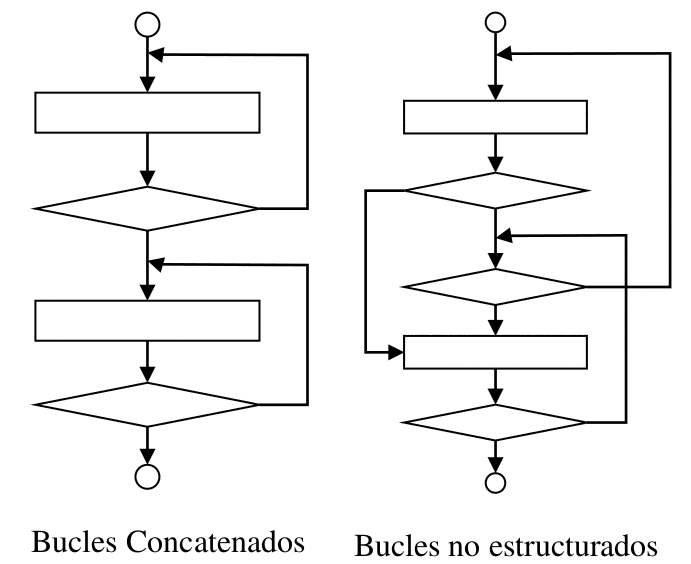
\includegraphics[width=0.5\linewidth]{Resources/Tema6/Ejemplo_BucleNoEstructurado.png}
    \caption{Ejemplificación de dos bucles: el izquierdo se ajusta a la programación estructurada, mientras que el derecho no lo hace.}
\end{figure}

\subsection{Utilización de la complejidad ciclomática de \textit{McCabe}}

La métrica de \textit{McCabe} es un \textbf{indicador del número de caminos independientes que existen en un grafo}; dicho de otro modo, trata de determinar, dado un grafo, cuántos caminos son precisos para probarlo. Se basa en la teoría de grafos. Por extensión, esta métrica también proporciona una medida cuantitativa de la complejidad lógica del módulo de software que se está probando.\\

El propio \textit{McCabe} definió como un buen criterio de prueba la consecución de la ejecución de un conjunto de caminos independientes igual al indicado por la métrica; es más, la métrica de \textit{McCabe} coincide con el número máximo de caminos independientes que puede haber un grafo. Cabe destacar que \textbf{un camino es independiente de otros si incorpora un arco que los demás no incluyen}.\\

Además, el conjunto de caminos que permite establecer asegura que todo el código de ejecuta, al menos una vez, por lo que cubriría la cobertura de sentencias. Este criterio también se ha propuesto como equivalente a la cobertura de decisiones, pero han surgido contraejemplos que lo invalidan.\\

La complejidad de \textit{McCave} $V (G)$ puede ser calculada de tres maneras a partir de un grafo de flujo $G$::
\begin{enumerate}
    \item $V (G) = a-n+2$, siendo $a$ el número de arcos, y $n$ el de nodos.
    \item $V (G) = r$, siendo $r$ el número de regiones cerradas del grafo.
    \item $V (G) = c+1$, siendo $c$ el número de nodos de condición. Una condición de $n$ arcos de salida se contabiliza cono $n-1$ (si $n>2$, equivale al número de bifurcaciones binarias necesarias para simular dicha bifurcación \textit{n-aria}).
\end{enumerate}

\begin{figure}[H]
    \centering
    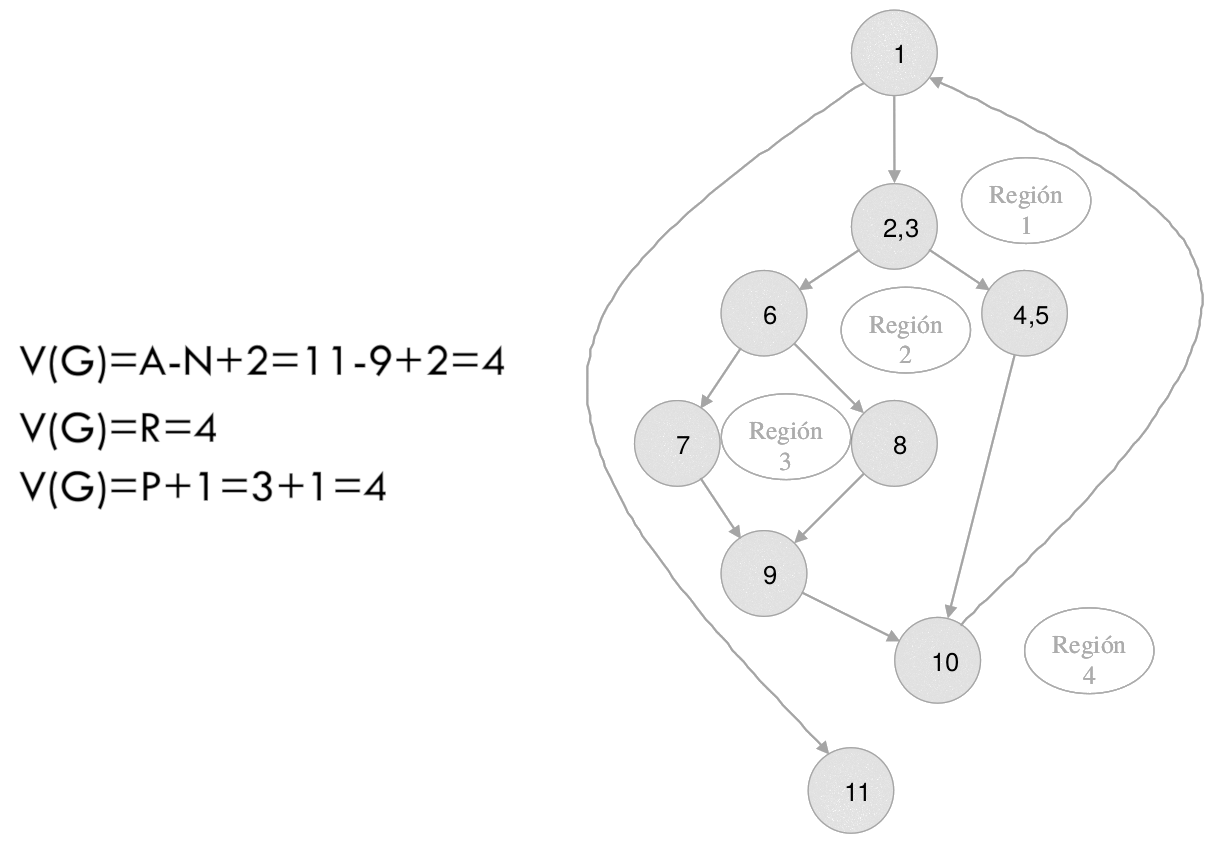
\includegraphics[width=0.9\linewidth]{Resources/Tema6/Ejemplo_McCabe.png}
    \caption{Ejemplificación del cálculo de la complejidad ciclomática de \textit{McCabe}.}
\end{figure}

\textbf{Nota:} \textit{Hay que tener presente, para el número de regiones, que la fórmula solo es aplicable a grafos fuertemente conexos (siempre existe un camino para cualesquiera dos nodos que se escojan). Esto no se verifica en los programas con un nodo de inicio y otro de final, por lo que, para calcular las regiones, deben unirse estos nodos, o bien debe contabilizarse la región externa.}\\

Una vez calculado del valor de $V (G)$, permitiendo afirmar por lo tanto el número máximo de caminos independientes del grafo $G$, para ayudar a la elección de los caminos de prueba, McCabe propone el \textbf{método del camino básico} para la selección de los caminos independientes. Consiste en:

\begin{enumerate}
    \item Se escoge un camino de prueba típico (básico).
    \item Se crean variaciones sobre el camino, de forma que cada una de ellas se distinga en, al menos, una arista de las demás.
    \item Una vez seleccionados los caminos, se analiza el código para determinar las entradas que los fuerzan.
    \item Finalmente, se revisa la especificación para precedir las salidas correctas (en teoría) ante las entradas determinadas.
\end{enumerate}

Es conveniente tener presente que algunos caminos no se podrán ejecutar solos, sino que requerirán la ejecución de algún otro. Además es posible que, para un camino, no exista un conjunto de entradas que lo fuercen, por lo que deberá ser sustituido por otro para seguir satisfaciendo el criterio de \textit{McCabe}.\\

\textbf{Nota:} \textit{$V (G)$ marca un límite mínimo de número de casos de prueba para un programa. Si $V (G)$ es mayor que 10, la probabilidad de encontrar defectos en el módulo aumenta por presentar una elevada complejidad (salvo que sea debido a sentencias \textit{switch case} o similares); en estos casos, debería replantearse el diseño del módulo.}


\section{Pruebas funcionales (de caja negra)}

Estas pruebas se centran en el estudio de la especificación del software; es decir, conocidas las entradas, es posible determinar las salidas esperadas, y el flujo de datos interno no importa. Se tratará de encontrar errores en las siguientes categorías mediante las pruebas de caja negra:

\begin{itemize}
    \item Funciones incorrectas o ausentes.
    \item Errores de interfaz.
    \item Errores en estructuras de datos o accesos a bases de datos.
    \item Errores de rendimiento.
    \item Errores de inicialización y terminación.
\end{itemize}

De nuevo, la prueba exahustiva es generalmente impracticable, por lo que deben buscarse criterios que permitan elegir un subconjunto de casos cuya ejecución aporte una cierta confianza en detectar los posibles defectos del software.\\

Existen dos enfoques a la hora de seleccionar casos de prueba de caja negra.

\subsection{Enfoque sistemático}

El diseño de pruebas se apoyará en las siguientes dos definiciones de \textit{Myers} para buscar \uline{buenos casos de prueba} (presenta una alta probabilidad de detectar un nuevo error):

\begin{itemize}
    \item El caso ejecuta el máximo número de posibilidades de entrada diferentes para reducir así el total de casos.
    \item Cada entrada cubre un conjunto extenso de otras: Además de dar información sobre la ausencia o presencia de defectos con las entradas probadas, estos resultados pueden ser generalizados con cierta seguridad para otro conjunto de entradas similares que no hayan sido probadas.
\end{itemize}

\subsubsection{Partición o clases de equivalencia}

Esta técnica de diseño de casos se basa en \textbf{dividir el dominio de valores de entradas} en un número finito de clases, de modo que \textbf{la prueba de un valor representativo de una clase permite suponer}, razonablemente, que \textbf{el resultado obtenido será el mismo} que el obtenido probando cualquier otro valor de la clase.\\

Para ello, hay que realizar las siguientes tareas:

\begin{enumerate}
    \item \textbf{Identificar las posibles clases de equivalencia a partir de la especificación del programa}. Consta de los siguientes pasos:
    
    \begin{enumerate}[a.]
        \item \textbf{Identificar las condiciones de las entradas del programa}; es decir, las restricciones de formato y posibles valores de las entradas.
        
        \item \textbf{Identificar, a partir de ellas, las clases de equivalencia}, que pueden ser (1) de datos válidos, o (2) de datos no válidos o erróneos. Esta identificación debe realizarse, como ya se comentó, basándose en el principio de igualdad de tratamiento de los valores de cada clase.\\
        
        Existen algunas \uline{reglas} que ayudan a identificar clases:

        \begin{enumerate}[R1.]
            \item Si se especifica un rango de valores, se creará una clase válida y dos clases no válidas. \textit{Por ejemplo, $5<n<7$.}
            \item Si se especifica una lista de valores de tamaño variable, se creará una clase válida y dos no válidas. \textit{Por ejemplo, puede haber de 1 a 4 titulares para una cuenta bancaria.}
            \item Si se especifica una situación del tipo \textit{debe ser} o booleana, se creará una clase válida y una no válida. \textit{Dos ejemplos serían que (1) el primer carácter debe ser una letra, o que (2) la edad debe introducirse en formato numérico.}
            \item Si se especifica un conjunto de valores admitidos, que son tratados de forma distinta, se creará una clase válida por cada valor, y una clase no válida. \textit{Por ejemplo, pueden registrarse tres tipos de inmuebles, siendo chalets, pisos, o locales comerciales.}
            \item En cualquier caso, si se sospoecha que ciertos elementos de una clase no se tratan igual que el resto de la misma, deben dividirse en clases menores.
        \end{enumerate}
    \end{enumerate}

    \item \textbf{Crear los casos de prueba correspondientes}. Consta de las siguientes fases:
    
    \begin{enumerate}[a.]
        \item Asignar un número único a cada clase de equivalencia.
        \item Hasta que todas las clases de equivalencia hayan sido cubiertas por casos de prueba, se tratará de escribir un caso que cubra tantas clases válidas no incorporadas como sea posible.
        \item Hasta que todas las clases de equivalencia no válidas hayan sido cubiertas, se escribe un caso para cada una de las clases no válidas sin cubrir.\\
        
        El motivo de cubrir, con casos individuales, las clases no válidas, es que \uline{ciertos controles de entrada pueden enmascarar o invalidar} otros controles similares. Por ejemplo, en un programa donde hay que \textit{introducir cantidad (1--99) y letra inicial (A--Z)}, ante el caso \textit{105} \texttt{\&} (dos errores), se puede indicar solo el mensaje \textit{105 fuera de rango}, y dejar sin examinar el resto de la entrada a pesar de ser también inválida. Esto sería incluso más peligroso si el programa respondiese con un mensaje ambiguo, como \textit{dato incorrecto, introduzca valor}, dado que podría llevar a pensar al equipo de pruebas a que ambos errores fueron correctamente identificados.
    \end{enumerate}
\end{enumerate}

\subsubsection{Análisis de valores límite (ALV)}

Mediante la experiencia, se ha podido constatar que los \textbf{los casos de prueba que exploran las condiciones límite de un programa producen un mejor resultado para la detección de defectos}. Las condiciones límite se pueden definir como \uline{las situaciones que se hayan directamente arriba, abajo, y en los márgenes de las clases de equivalencia}.\\

Realmente, esta técnica de diseño de casos complementa a la de particiones. Las diferencias entre ellas son:

\begin{itemize}
    \item En lugar de elegir ``cualquier'' elemento como representativo de una clase de equivalencia, se requiere que se escojan uno o más elementos tal que los márgenes se somentan a prueba.
    \item En lugar de concentrarse únicamente en el dominio de entradas, los casos de prueba se generan considerando también el espacio de salida.
\end{itemize}

De nuevo, el proceso de selección es heurístico, como en la técnica de particiones, pero existen ciertas reglas orientativas:

\begin{enumerate}[R1.]
    \item Si una condición de entrada especifica un intervalo cerrado de valores (\textit{por ejemplo $[-1.0, 1.0]$}), se deben generar casos para los extremos del rango (\textit{$-1.0$ y $1.0$}), y casos no válidos para situaciones justo más allá de los extremos (\textit{$-1.001$ y $1.001$, en el caso de que se admitan tres decimales}).
    \item Si la condición de entrada especifica un número de valores (oir ejemplo, \textit{el fichero de entrada tendrá de 1 a 255 registros}), se diseñarán casos para (1) el valor máximo, (2) el valor mínimo, (3) uno más que el máximo, y (4) uno menos que el mínimo (\textit{en este caso, $0, 1, 255, 256$}).
    \item Usar la regla R1 para la condición de salida. \textit{Por ejemplo, si el descuento máximo aplicable en una compra será el 50\%, y el mínimo será el 6\%, se escribirán casos para intentar obtener descuentos de 5.99\%, 6\%, 50\%, y 50.01\%}.
    \item Usar la regla R2 para cada condición de salida. \textit{Por ejemplo, si el programa puede mostrar de 1 a 4 listados, se escribirán casos para intentar generar 0, 1, 4, y 5 listados.}\\
    En esta regla, como en la R3, debe recordarse que:
    \begin{itemize}
        \item Los valores límite de entrada no generan necesariamente los valores límite de salida.
        \item No siempre se pueden generar resultados fuera del rango de salida, pero debe ser considerado igualmente.
        \item Si la entrada o salida de un programa es un conjunto ordenado, los casos deben concentrarse en el primer y último elemento. \textit{Por ejemplo, una tabla, o un archivo secuencial.}
    \end{itemize}
\end{enumerate}

\subsubsection{Conjetura de errores}

La idea básica de esta técnica consiste en \textbf{enumerar una lista de equivocaciones que pueden cometer los desarrolladores}, para después generar casos de prueba por cada uno de los elementos en ella. No existen directivas eficaces, ya que la lista será creada en base a la intuición y la experiencia; sin embargo, algunos valores a tener en cuenta son:

\begin{itemize}
    \item El valor cero, tanto en la entrada como en la salida.
    \item En situaciones en las que se introduce un número variable de valores, conviene centrarse en los casos de (1) que no haya ningún valor, (2) que solo haya uno, y (3) que todos los valores sean iguales.
    \item Es recomendable imaginar que el programador puediera haber interpretado algo mal en la especificación.
    \item También interesa imaginar lo que el usuario pueda introducir como entrada a un programa, previniendo toda clase de acciones, incluse como si fuese poco hábil, o que presentase malas intenciones.
\end{itemize}

\subsection{Enfoque aleatorio}

Se basa en la generación de pruebas aleatorias, en las cuales se simula la entrada habitual del programa creando los datos de entrada en la secuencia y frecuencia con las que podrían aparecer en la práctica. Generalmente, el objetivo de estos llamados \uline{tests de esfuerzo} es el \textbf{evaluar el rendimiento del sistema}, puesto que, como las entradas son generadas aleatoriamente, no se pueden precedir las salidas. Esto es debido a que, si por el contrario contásemos con un software que predijese las salidas con total fiabilidad, este podría reemplazar directamente al software que está siendo probado.\\

Para crear estos tests, es necesario contar con una herramienta generadora de pruebas, a la que se especifica la descripción de las entradas, las secuencias de entrada posibles, y las probabilidades de ocurrir en la práctica (por ejemplo, indicando una distribución estadística si la siguen). Si el proceso de generación se ha realizado correctamente, eventualmente se crearán todas las posibles entradas del programa, en todas las posibles combinaciones y permutaciones. 

\subsection{Métodos de prueba basados en grafos}

El primer paso en la prueba de caja negra es \textbf{entender los objetos que se modelan en el software}, y las relaciones entre ellos. Una vez realizado todo esto, se continúa definiendo una serie de pruebas que verifiquen que \uline{todos los objetos tienen, entre ellos, las relaciones esperadas}. Dicho de otra manera, la prueba del software empieza creando un grafo de objetos importantes y sus relaciones, y después \textbf{diseñando una serie de pruebas que cubran el grafo de manera que se ejerciten todos los objetos y sus relaciones} para descubrir los errores.\\

Para llevar a cabo estos pasos, debe comenzarse creando el grafo, que representará:

\begin{itemize}
    \item Objetos mediante sus nodos.
    \item Relaciones entre los objetos mediante los arcos.
    \item Propiedades de un objeto mediante el peso de su correspondiente nodo.
    \item Características de las relaciones mediante el peso de su correspondiente arco.
\end{itemize}

\begin{figure}[H]
    \centering
    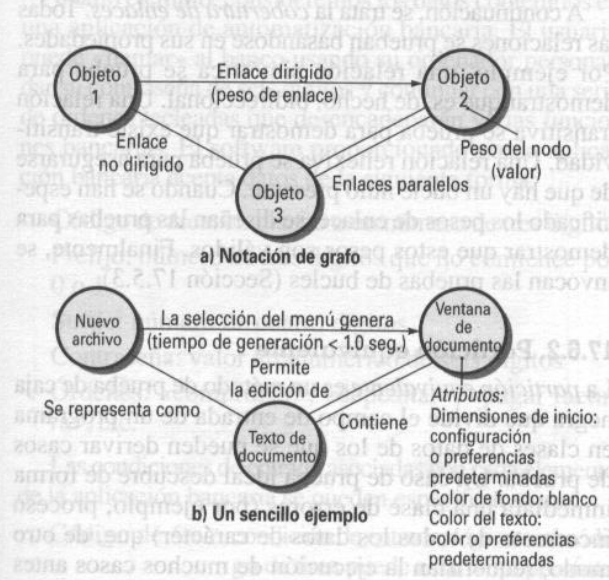
\includegraphics[width=0.5\linewidth]{Resources/Tema6/Ejemplo_Grafo.png}
    \caption{Representación simbólica de un grafo para pruebas de caja negra.}
    \label{fig:estrategiasPruebas}
\end{figure}

Una vez creado el grafo, se puede proceder a la creación de los casos de prueba. Entre los beneficios que estos grafos a este procedimiento, se encuentra el facilitar:

\begin{itemize}
    \item La identificación de los bucles a probar.
    \item El cumplimiento de la cobertura de nodos, de modo que ninguno haya sido omitido.
    \item El cumplimiento de la cobertura de enlace, probándose todas y cada una de las relaciones. Cada relación debe ser probada basándose en sus propiedades:
    \begin{itemize}
        \item Se estudia la transitividad de las relaciones secuenciales para determinar cómo se propaga el impacto de las relaciones a través de los objetos definidos en el grafo.
        \item La simetría de una relación también es importante para el diseño de casos de prueba; si un enlace es bidireccional, debería probarse esta característica.
        \item Todos los nodos del grafo deberían ser reflexivos, es decir, tener una relación que los devuelva a ellos mismos. % No estoy seguro, ya estaba escrito por el autor original, y los apuntes no profundizan en ello.
    \end{itemize}
\end{itemize}

A continuación, se describe un número de métodos de prueba de comportamiento que pueden hacer uso de los grafos:

\begin{itemize}
    \item \textbf{Modelado del flujo de transacción:} Los nodos representan los pasos de alguna transacción, y los enlaces son las conexiones lógicas entre ellos; sería posible partir de un DFD. \textit{Por ejemplo, los pasos requeridos para hacer una reserva en un hotel; son pasos del proceso, se use software o no.}
    \item \textbf{Modelado de estados finitos:} Los nodos son estados del software observables por el usuario, y los enlaces representan las transiciones que ocurren para movese de un estado a otro. \textit{Por ejemplo, el usuario puede interactuar con pantallas, sobre las cuales realizar acciones que lleven a otras pantallas.}
    \item \textbf{Modelado del flujo de datos:} Los nodos son objetos de datos, y los enlaces son las transformaciones que sufren para pasar de ser un objeto a otro.
\end{itemize}

Es importante tener presente que \textbf{todos son modelos de caja negra}, por lo que no modelan cómo está programado el software; es decir, no modelan ni los estados del software, ni sus transacciones programadas, ni sus flujos de datos. En realidad, \textbf{modelan su comportamiento visible}.


\section{Enfoque práctico recomendado para el diseño de casos}

El enfoque remonendado para el uso de las técnicas de diseño de casos pretende mostrar el uso más apropiado de cada técnica para la obtención de un conjunto de casos útiles sin perjuicio de las estrategias de niveles de prueba.

\begin{enumerate}
    \item \textbf{Si la especificación contiene combinaciones de condiciones de entrada, se comienza formando sus grafos causa--efecto} para comprenderlas con más facilidad.
    \item \textbf{Se identifican las clases válidas y no válidas de equivalencia para la entrada y la salida}.
    \item En todos los casos, \textbf{se usa el análisis de valores límite (AVL) para añadir casos de prueba}: Elegir límites para dar valores a las causas en los casos generados, asumiendo que cada caso es una clase de equivalencia.
    \item \textbf{Se utiliza la conjetura de errores para añadir nuevos casos}, principalmente referidos a valores especiales.
    \item \textbf{Se ejecutan los casos generados hasta el momento (de caja negra), y se analiza la cobertura obtenida}.
    \item \textbf{Se examina la lógica del programa para añadir los casos precisos (de caja blanca) para cubrir el criterio de cobertura elegido}, siempre y cuando no haya sido satisfecho en el anterior punto.
\end{enumerate}


\section{Documentación del diseño de las pruebas (IEEE 829)}

Conviene tener siempre presente que \textbf{la documentación de las pruebas es necesaria para una buena organización de las mismas, así como para asegurar su reutilización}. Según el estándar \textbf{estándar IEEE 829}, se generará la siguiente documentación:

\begin{figure}[H]
    \centering
    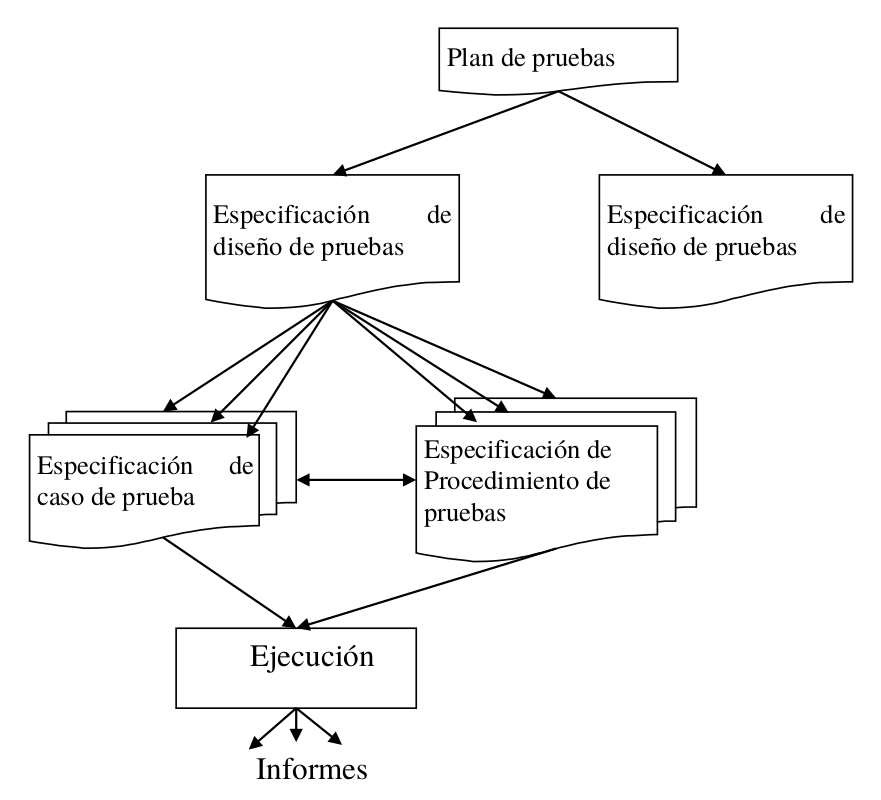
\includegraphics[width=0.6\linewidth]{Resources/Tema6/IEEE_829.png}
    \caption{Representación de los documentos del estándar IEEE 829 para la documentación del diseño de pruebas.}
    \label{fig:IEEE829}
\end{figure}

\begin{enumerate}
    \item \textbf{Plan de pruebas}: El documento tiene el objetivo de mostrar la planificación general del esfuerzo para cada fase de la estrategia de prueba del producto. Parte de los elementos fijados en el estándar son:
    \begin{enumerate}
        \item Una introducción y resumen de los elementos y características a probar.
        \item Los elementos de software a probar (programas o módulos).
        \item Qué características se van a probar y cuáles no.
        \item Actividades, técnicas, herramientas\ldots
        \item Criterios de paso/fallo para cada elemento.
        \item Documentos a entregar.
        \item Actividades de preparación y ejecución de las pruebas.
        \item Necesidades del entorno.
        \item Responsables de la realización de las pruebas, y sus necesidades.
        \item Esquema de tiempos y riesgos asumidos.
    \end{enumerate}

    \item \textbf{Especificación del diseño de pruebas}): Partiendo del plan de pruebas, se realizan ampliaciones de los detalles mostrados, especificando un diseño de prueba por cada módulo del programa. En el estándar se fija la siguiente estructura:
    \begin{enumerate}
        \item Las características a probar de los elementos sofware.
        \item Detalles sobre el plan de pruebas creado, incluyendo las técnicas de prueba específicas y los métodos de análisis de resultados.
        \item Se identifica cada prueba: Identificador, casos que se van a utilizar, procedimientos que se van a seguir.
        \item Criterios de paso/fallo de la prueba.
    \end{enumerate}

    \item \textbf{Especificación del caso de prueba}: A partir del anterior diseño, se definen con detalle cada uno de los casos de prueba mencionados, especificando datos de pruebas exactos, resultados esperados, y demás detalles, para obtener un conjunto de pruebas de validación y de verificación. En el estándar se fija la siguiente estructura:
    \begin{enumerate}
        \item Elementos software a probar, y cuáles de sus características serán ejercitadas por el caso.
        \item Especificaciones de cada entrada requerida para ejecutar el caso. Deben detallarse además las relaciones entre estas; \textit{por ejemplo, la sincronización de las mismas.}
        \item Especificaciones de todas las salidas y las características requeridas (\textit{por ejemplo, el tiempo de respuesta}).
        \item Necesidades del entorno. \textit{Por ejemplo, en cuanto a hardware, software, o personal}.
        \item Requisitos o restricciones especiales de procedimiento.
        \item Dependencias entre casos.
    \end{enumerate}

    \item \textbf{Especificación del procedimiento de prueba} (\textit{}): Tras generar los casos de prueba detallados, se especifica cómo proceder en detalle a su ejecución. En el estándar se fija la siguiente estructura:
    \begin{enumerate}
        \item Objetivo del procedimiento y lista de casos que se ejecutan con él.
        \item Requisitos especiales para la ejecución.
        \item Pasos en el procedimiento. Además de la manera de registrar los resultados y los incidentes de la ejecución, se debe especificar:
        \begin{itemize}
            \item La secuencia necesaria de acciones para preparar la ejecución.
            \item Acciones necesarias para empezar la ejecución.
            \item Acciones necesarias durante la ejecución.
            \item Cómo se realizarán las medidas. \textit{Por ejemplo, del tiempo de respuesta.}
            \item Cómo tratar incidencias y restaurar el entorno de ejecución.
        \end{itemize}
    \end{enumerate}
\end{enumerate}


\section{Ejecución de las pruebas}

\subsection{El proceso de ejecución (IEEE 1008)}

El proceso abarca las siguientes fases:

\begin{figure}[H]
    \centering
    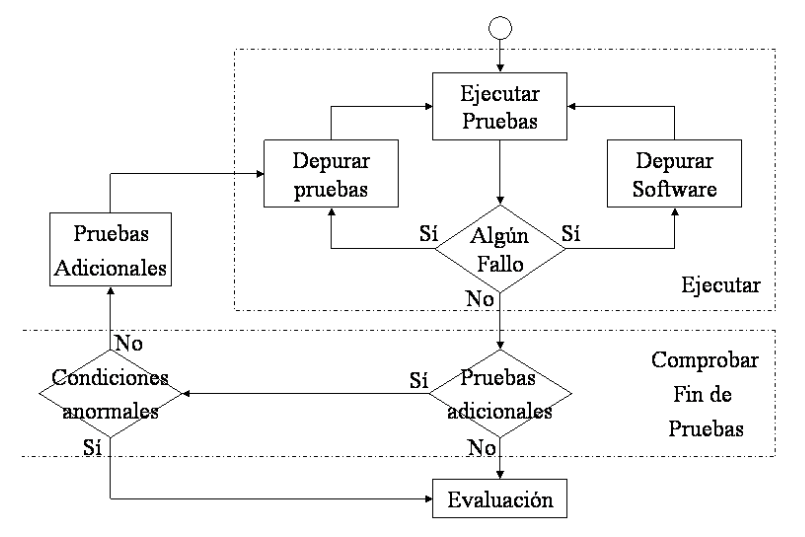
\includegraphics[width=0.75\linewidth]{Resources/Tema6/IEEE_1008.png}
    \caption{Representación de proceso de pruebas según el estándar IEEE 1008.}
\end{figure}

\begin{enumerate}
    \item \textbf{Proceso de ejecución}: Se ejecutan las pruebas, cuyos casos y procedimientos han sido ya diseñdos previamente. Consta de las siguientes fases:
    \begin{enumerate}
        \item Se ejecutan las pruebas.
        \item Se comprueba si ha habido algún fallo al ejecutar, que impida terminar la ejecución de algún caso. \textit{Por ejemplo, se cae el sistema, se bloquea el teclado\ldots}
        \item Si lo ha habido, se puede deber a un defecto software, que llevará a la depuración o corrección del código, o a un defecto en el propio diseño de las pruebas. En ambos casos, \uline{las nuevas pruebas o las corregidas deberán ejecutarse}.
        \item De no existir fallo, se pasará a la comprobación de la terminación de las pruebas.
    \end{enumerate}

    \item \textbf{Comprobación de la conclusión del proceso de prueba}: Se lleva a cabo según criterios de compleción de prueba que suelen ser especificados en el plan de pruebas. Consta de las siguientes fases:
    \begin{enumerate}
        \item Tras la ejecución, se comprobará si se cumplen los criterios de compleción descritos en el correspondiente plan de pruebas. \textit{Por ejemplo, se terminan las pruebas cuando se han probado todos los procedimientos de operación o se ha cumplido la cobertura lógica marcada.}
        \item En caso de terminar las pruebas, se pasa a la evaluación de los productos probados sobre la base de los resultados obtenidos. \textit{Se alcanza una terminación normal.}
        \item En caso de no terminar las pruebas, se debe comprobar la presencia de condiciones anormales en la prueba. Si hubiesen existido condiciones anormales (\textit{por ejemplo, no se han podido ejecutar todos los casos porque el sistema se cae regularmente}), se pasa de nuevo a la evaluación; \textit{se alcanza una terminación anormal}. En caso contrario, se pasa a generar y ejecutar pruebas adicionales para satisfacer cualquiera de las dos terminaciones.
    \end{enumerate}
    \item \textbf{Si las pruebas han terminado, se evalúan los resultados; en caso contario, hay que generar pruebas adicionales} para que se satisfagan los criterios de compleción de pruebas.
\end{enumerate}

\subsection{Documentación de la ejecución de las pruebas}

La documentación de la ejecución de las pruebas también es fundamental para dejar constancia de los resultados de las pruebas. \uline{Parte de los documentos generados se relacionan directamente con el estándar IEEE 829}, pudiéndose distinguir dos grupos principales:

\begin{itemize}
    \item \textbf{Documentación de entrada}: Constituida principalmente por las especificaciones de los casos de prueba que se van a usar, y las especificaciones de los procedimientos de pruebas.
    
    \item \textbf{Documentación de salida o informes sobre la ejecución}: Cada ejecución generará dos tipos de documentos.
    \begin{itemize}
        \item \textbf{Histórico de pruebas} (\textit{test log}): Documenta todos los hechos relevantes ocurridos durante la ejecución de las pruebas. La estructura fijada en el estándar es:
        \begin{itemize}
            \item Descripción de la prueba, detallando los elementos probados y el entorno de prueba.
            \item Anotaciones de datos sobre cada hecho ocurrido, incluidos el inicio y fin de la prueba: fecha, hora, e identificador del informe de incidente asociado, en caso de haberlo.
            \item Otras informaciones.
        \end{itemize}
        \item \textbf{Informes de los incidentes ocurridos} (\textit{test incident report}), siempre en caso de que sucedan durante la ejecución: Cada uno documenta un incidente que requirá una posterior investigación. La estructura fijada en el estándar es:
        \begin{itemize}
            \item Resumen del incidente.
            \item Descripción de datos objetivos: fecha, hora, entradas, resultados esperados, etc.
            \item Impacto que tendrá sobre las pruebas.
        \end{itemize}
    \end{itemize}
    Además, \textbf{toda la documentación de salida correspondiente a un mismo diseño de prueba se recoge en un informe resumen de pruebas} (\textit{test summary report}), resumiéndose así los resultados de las actividades de prueba, y \uline{aportándose una evaluación del software} basada en ellos. Entre otros elementos a incluir en el informe, destacan:
    \begin{itemize}
        \item Resumen de la evaluación de los elementos probados.
        \item Variaciones del software respecto a su especificación de diseño, así como las variaciones en las pruebas.
        \item Valoración de la extensión de la prueba. \textit{Cobertura lógica, funciona, de requisitos, etc.}
        \item Resumen de cada una de las actividades de prueba, incluyendo detalles sobre los recursos empleados.
    \end{itemize} 
\end{itemize}

\textbf{Nota:} \textit{Cada uno de los documentos detallados anteriormente, tanto para la documentación del diseño de las pruebas, como para la ejecución de estas, debe contar con un identificador.}

\subsection{Depuración}
La depuración es el \textbf{proceso de localizar, analizar y corregir los defectos que se sospecha que contiene el software}. Suele ser la consecuencia de una prueba con éxito, que conlleva mandar un módulo a depuración. De este modo, el proceso de depuración puede \uline{dar lugar a dos situaciones}:

\begin{itemize}
    \item \textbf{Encontrar la causa del error, analizarla y corregirla}.
    \item \textbf{No encontrar la causa} y, por lo tanto, tener que \textbf{generar nuevos casos de prueba que puedan proporcionar información adicional} para su localización.
\end{itemize}

Por lo tanto, se puede distinguir las \uline{dos fases} siguientes:

\begin{itemize}
    \item \textbf{Localización del defecto}: Suele conllevar la mayor parte del esfuerzo.
    \item \textbf{Corrección del defecto}.
\end{itemize}

Además, tras corregir el efecto, \uline{deberán efectuarse nuevas pruebas que comprueben si efectivamente ha sido eliminado}.

\begin{figure}[H]
    \centering
    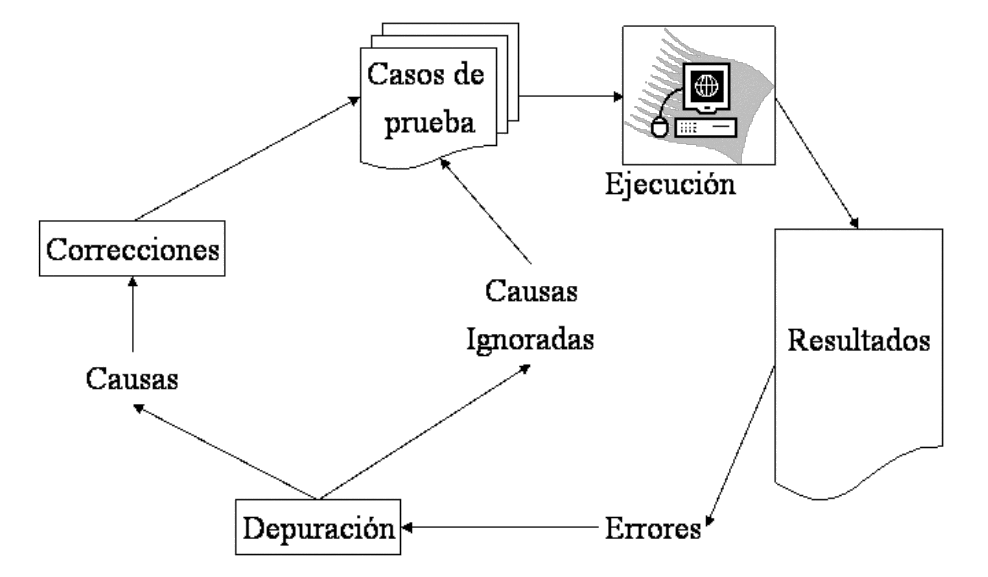
\includegraphics[width=0.7\linewidth]{Resources/Tema6/ProcesoDepuracion.png}
    \caption{Representación de proceso de depuración.}
\end{figure}

\subsubsection{Consejos para la depuración}

\begin{itemize}
    \item \textbf{Para la localización del error:}
    \begin{itemize}
        \item Es el proceso mental de solución de un problema. Por ello, debería analizarse la información disponible, en lugar de explorar aleatoriamente o experimentar cambiando el programa.
        \item Las herramientas de depuración deberían emplearse como recurso secundario.
        \item Al llegar a un punto muerto, puede merecer la pena pasar a otra cosa para refrescar la mente, e incluso puede ayudar el describir el problema a otra persona.
        \item Se deben atacar los errores individualmente, o solo se dificultará la depuración.
        \item Se debe fijar la atención también en los datos manejados, y no solo en la lógica del proceso.
    \end{itemize}

    \item \textbf{Para la corrección del error:}
    \begin{itemize}
        \item Donde hay un defecto, suele haber más (\textit{ejemplo del principio de Pareto}).
        \item Debe corregirse el defecto, en lugar de intentar enmascarar sus síntomas.
        \item La probabilidad de corregir un defecto perfectamente no es el 100\%, por lo que las correciones deben ser revisadas antes de implatarlas.
        \item Debe tenerse cuidado para no crear nuevos defectos por corregir sin cautela.
        \item La corrección debe situarnos temporalmente en la fase de diseño, para alterar el correspondiente al código defectuoso.
    \end{itemize}
\end{itemize}

\subsection{Análisis de errores a análisis causal}

El objetivo del análisis causal es \textbf{proporcionar información sobre la naturaleza de los defectos, para que así el personal pueda prevenirlos en el futuro}, al conocer los errores que comete; esta información no debe ser empleada nunca para evaluar al personal. Se recoge la siguiente información:
\begin{itemize}
    \item Cuándo se cometió.
    \item Quién lo cometió.
    \item Qué se hizo mal.
    \item Cómo se podría haber prevenido.
    \item Por qué no se detectó antes.
    \item Cómo se podría haber detectado antes.
    \item Cómo se encontró el error.
\end{itemize}


\section{Estrategia de aplicación de las pruebas}

Una vez conocidas las técnicas de diseño y de ejecución, se debe analizar \uline{cómo se plantea la utilización de las pruebas en el ciclo de vida}. La estrategia de aplicación y la planificación de las pruebas pretenden \uline{integrar el diseño de los casos de prueba y permite la coordinación del personal y del cliente}, gracias a la definición de los papeles que deben desempeñar cada uno de ellos, así como de la forma de llevarlos a cabo.\\

Las etapas de las que constaría la estragia serían:

\begin{figure}[H]
    \centering
    \includegraphics[width=0.7\linewidth]{Resources/enfoquePruebas}
    \caption{Las diferentes estrategias de prueba y su relación con las otras fases del construcción del software}
    \label{fig:estrategiasPruebas}
\end{figure}

\begin{enumerate}
    \item \textbf{Se comienza en la prueba de cada módulo}, realizada normalmente por el propio personal de desarrollo.
    \item Con el esquema del diseño del software, \textbf{los módulos probados se integran para comprobar sus interfaces}.
    \item \textbf{El software totalmente ensamblado se prueba como un conjunto} para comprobar si cumple o no tanto los requisitos funcionales como los requisitos de rendimientos, seguridad, etc. Este nivel \uline{coincide con la prueba del sistema cuando solo se trata de software}.
    \item El caso de que el sistema final coste de más que software, \textbf{el software ya validado se integra con el resto del sistema} (\textit{por ejemplo, elementos mecánicos}), \textbf{para probar su funcionamiento conjunto}. \textit{Por extensión, todavía es posible simular el hardware implicado en la anterior etapa. El resultado de esta fase es la certeza de haber hecho lo deseado, además de haberlo hecho bien.}
    \item Finalmente, \textbf{el producto final se pasa a la prueba de aceptación par que el usuario compruebe, en su propio entorno de explotación si lo acepta o no}. \textit{El resultado de esta fase es que el usuario tenga la certeza de recibir lo que él quería}.
\end{enumerate}

Como se puede ver, \uline{cada nivel de prueba se centra en probar el software en referencia al trabajo realizado en una diferente etapa de desarrollo}.

\textbf{Nota:} \textit{Las pruebas de aceptación, de sistema y de integración están relacionadas directamente con las pruebas de validación. Por otra parte, las pruebas de integración (se encuentra en ambos bandos) y de unidad se encuentran directamente relacionadas con las pruebas de verificación. De todos modos, una prueba de módulo puede centrarse también en la especificación de las funciones que este debe realizar (de caja negra).}\\

\textbf{Nota:} \textit{A pesar de que un ciclo en cascada tenga una fase de pruebas, estas suelen distribuirse a lo largo del todo el ciclo de vida.}\\


\section{Pruebas en desarrollos orientados a objetos (\textit{OO})}

Las técnicas y estrategias presentadas hasta el momento están inspiradas en la aplicación a desarrollos estructurados. Por lo tanto, al trabajar con tecnología \textit{OO}, algunas de ellas pierden su interés o deben adaptarse.\\

\subsection{Punto de vista del diseño de casos de pruebas}

\begin{itemize}
    \item \textbf{Técnicas de caja negra}: Siguen siendo completamente válidas. \textit{Por ejemplo, el AVL, el tratamiento de combinaciones de entrada, la conjetura de errores\ldots} Los casos de prueba deberían ser diseñados basándose en:
          \begin{itemize}
              \item Los datos y eventos incluidos en los escenarios de los casos de uso.
              \item Los caminos que se pueden trazar en los diagramas de actividad, o en los de estados, que describan el caso, sin olvidar todos los flujos alternativos, ni los tratamientos de errores y excepciones.
          \end{itemize}
    \item \textbf{Técnicas de caja blanca}: Disminuyen sus posibilidades de aplicación, quedando confinadas a las instrucciones de cada método de cada clase. También cabría la posibilidad de aplicar la cobertura de caminos (incluido el criterio de \textit{McCabe}) no solo al código de los métodos, sino también a los diagramas de comportamiento con estructura de red; \textit{por ejemplo, diagramas de estados, de actividad, etc.}
\end{itemize}

En el caso del diseño de pruebas, cabe señalar además la posibilidad de \uline{distinguir criterios según el nivel de pruebas en el que se sitúe el diseño}. Así, para las pruebas de unidad (es decir, pruebas de clases), la prueba de clases de equivalencia y de AVL  son apropiadas aplicándolas a las entradas y salidas representadas como parámetros de métodos fundalmente. Sin embargo, \textbf{los cambios más radicales aparecen en las pruebas de integración}, dado que el enfoque de integración basado en la existencia de una estructura jerárquica no tiene sentido frente a las estructuras de colaboración en red definidas para el software \textit{OO}.\\

Por una parte, existen propuestas que permiten \uline{encontrar aquellas clases que dependen en su funcionamiento de sí mismas o solo de unas pocas clases, para tomarlas como destino de la primera oleada de pruebas de integración}, de modo que más adelante se irán sometiendo a prueba las clases que dependen solo de las ya probadas, y así consecutivamente hasta integrar toda la aplicación. Sin embargo, el enfoque más habitual consiste en \uline{ir probando hilos de clases que colaboran para una función o servicio del sistema}, seguramente definidos en diagramas de colaboración; los diagramas de estado pueden aportar una mayor información para el rigor de la prueba.

\subsection{Cuestiones a tener en cuenta}

Finalmente, se señalarán dos cuestiones que tienen una gran influencia en las pruebas de software \textit{OO}
Ciertas cuestiones a tener en cuenta a la hora de probar software orientado a objetos son:
\begin{itemize}
    \item \textbf{Herencia}: Probar un método de la clase padre no garantiza su funcionamiento en clases hijas.
    \item \textbf{Polimorfismo}: Un único método puede tener implementaciones diferentes en función de la clase en la que se use, empeorando la preocupación del anterior punto.
    \item También Es conveniente recordar que la propia programación o diseño \textit{OO} hace menos probables ciertos tipos de error y más probables otros, además de provocar la aparición de nuevos tipos de defectos, frente a los desarrollos estructurados.
\end{itemize}

\newpage
\section{Ejemplo práctico de cálculo de la complejidad ciclomática de un método}

\begin{figure}[H]
    \centering
    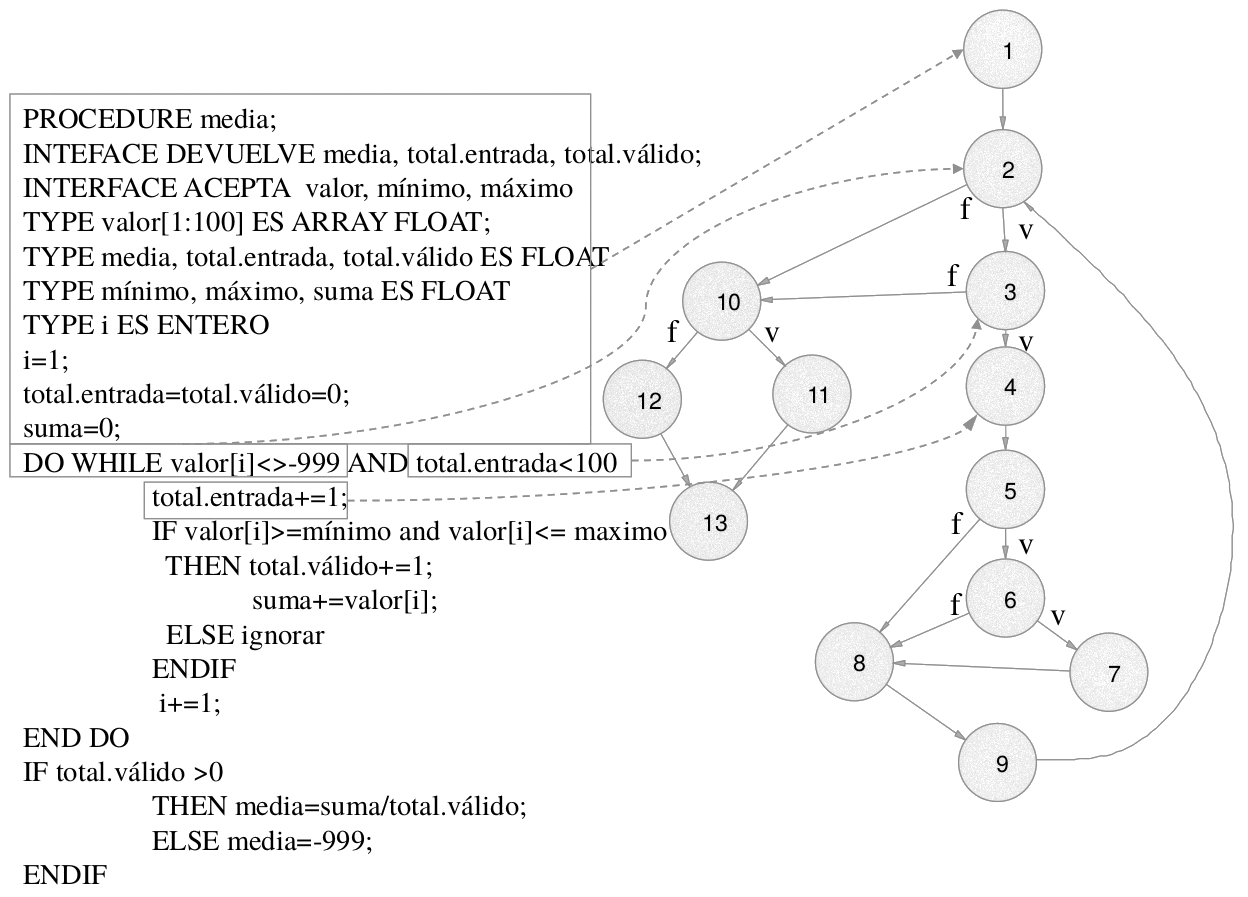
\includegraphics[width=0.9\linewidth]{Resources/Tema6/Ejemplo_CalculoComplejidadCiclomatica.png}
    \caption{Ejemplo de un método y su correspondiente grafo de flujo.}
\end{figure}

\paragraph{Complejidad de \textit{McCave}}

\begin{enumerate}
    \item $V (G) = a-n+2 = 17-13+2 = 6$.
    \item $V (G) = r = 6$.
    \item $V (G) = c+1 = 5+1 = 1$.
\end{enumerate}